\documentclass{beamer}
\usetheme{Gelugor}
\usepackage{hyperref}
\usepackage[utf8]{inputenc}
\usepackage[spanish]{babel}
\usepackage[default]{droidserif}
\title{Análisis y Diseño de Software}
\subtitle{Introducción a GitHub}
\author[Grupo1]{
Martha Suntaxi\\Johanna Paz\\Victor Jumbo\\Andre Montoya\\Wilson Iriarte
}
\date{\today}
\institute{Ingeniería en Sistemas\\}

\begin{document}
	
	%INICIO carátula
	\begin{frame}[plain,t]
		\titlepage
	\end{frame}
	%FIN carátula

	\section{Introducción a GitHub}

\subsection{Agenda}
\begin{frame}
\frametitle{Agenda}
{\small
\begin{itemize}
\item Introducción
	\begin{itemize}
	\item ¿Qué es GitHub?
	\item ¿Para que sirve?
	\item ¿Qué uso le daremos?
	\item ¿Qué herramientas proporciona?
	\end{itemize}
\item Instalación
\item Comandos Principales
	\begin{itemize}
	\item Comandos Básicos
	\item Trabajos con Ramas
	\item Acciones con Archivos
	\end{itemize}
\item Conclusiones
\end{itemize}}
\end{frame}
\subsection{Introducción}
		\begin{frame}
			\frametitle{Introducción}
			%\framesubtitle{Tema}
			\begin{center}
\includegraphics[width=2cm, height=3cm]{git.jpg}\end{center}
			\begin{center}\textbf{\Large ¿Qué es GitHub?}\end{center}
			GitHub es una plataforma de desarrollo colaborativo de software para alojar proyectos utilizando el 						sistema de control de versiones Git.\\
		\end{frame}
		\begin{frame}
			\frametitle{Introducción}
			%\framesubtitle{Tema}
			\begin{center}\textbf{\Large ¿Para que sirve?}\end{center}
			{\small \begin{itemize}
			\item Aloja tu repositorio de código y te brinda herramientas muy útiles para el trabajo en equipo, dentro 			de un proyecto.
			\item Se Puede contribuir a mejorar el software de los demás. Para poder alcanzar esta meta, GitHub provee 			de funcionalidades para hacer un fork y solicitar pulls.
			\end{itemize}\ \\
			Realizar un fork es simplemente clonar un repositorio ajeno (genera una copia en tu 						cuenta), para eliminar 	algún bug o modificar cosas de él. Una vez realizadas tus modificaciones puedes 					enviar un pull al dueño del proyecto. Éste podrá analizar los cambios que has realizado fácilmente, y si 				considera interesante tu contribución, adjuntarlo con el repositorio original.}
			\\
		\end{frame}
		\begin{frame}
			\frametitle{Introducción}
			%\framesubtitle{Tema}
			\begin{center}\textbf{\Large ¿Qué uso le daremos?}\end{center}
			{\small En nuestra especialidad “Programación”, fuimos aprendiendo cosas y creando programas de 							código abierto, fomentando el software libre.
			Podremos crear una cuenta gratuita y comenzar a subir repositorios de código (o crearlos desde 0), para 					que con la ayuda de todos ese proyecto mejore; así como también fortalecer los proyectos de los demás para 			crecer como grupo.}
		\end{frame}
		\begin{frame}
			\frametitle{Introducción}
			%\framesubtitle{Tema}
			\begin{center}\textbf{\Large ¿Qué herramientas proporciona?}\end{center}
			{\small En la actualidad, GitHub es mucho más que un servicio de alojamiento de código. Además de éste, se 			ofrecen varias herramientas útiles para el trabajo en equipo. Entre ellas, caben destacar:}
			{\footnotesize
			\begin{itemize}
			\item Una wiki para el mantenimiento de las distintas versiones de las páginas.
			\item Un sistema de seguimiento de problemas que permiten a los miembros de tu equipo detallar un problema 			con tu software o una sugerencia que deseen hacer.
			\item Una herramienta de revisión de código, donde se pueden añadir anotaciones en cualquier punto de un 				fichero y debatir sobre determinados cambios realizados en un commit específico.
			\item Un visor de ramas donde se pueden comparar los progresos realizados en las distintas ramas de 						nuestro repositorio.
			\end{itemize}}
		\end{frame}
\subsection{Instalación}
	\begin{frame}
			\frametitle{Instalación}
			%\framesubtitle{Tema}
			{\small
		\begin{itemize}
			\item {\textsf{Crear una cuenta en: }}\url{https://github.com/}
		\end{itemize}
		}
		\begin{center}
			
\includegraphics[width=8cm,height=5cm]{manual-img1.png}
		\end{center}
	\end{frame}
	\begin{frame}
		\frametitle{Instalación}
		\begin{itemize}
			\item {\sffamily Validar la Cuenta en su correo para poder acceder e instalar nuevos repositorios.}
		\end{itemize}
		\begin{center}
			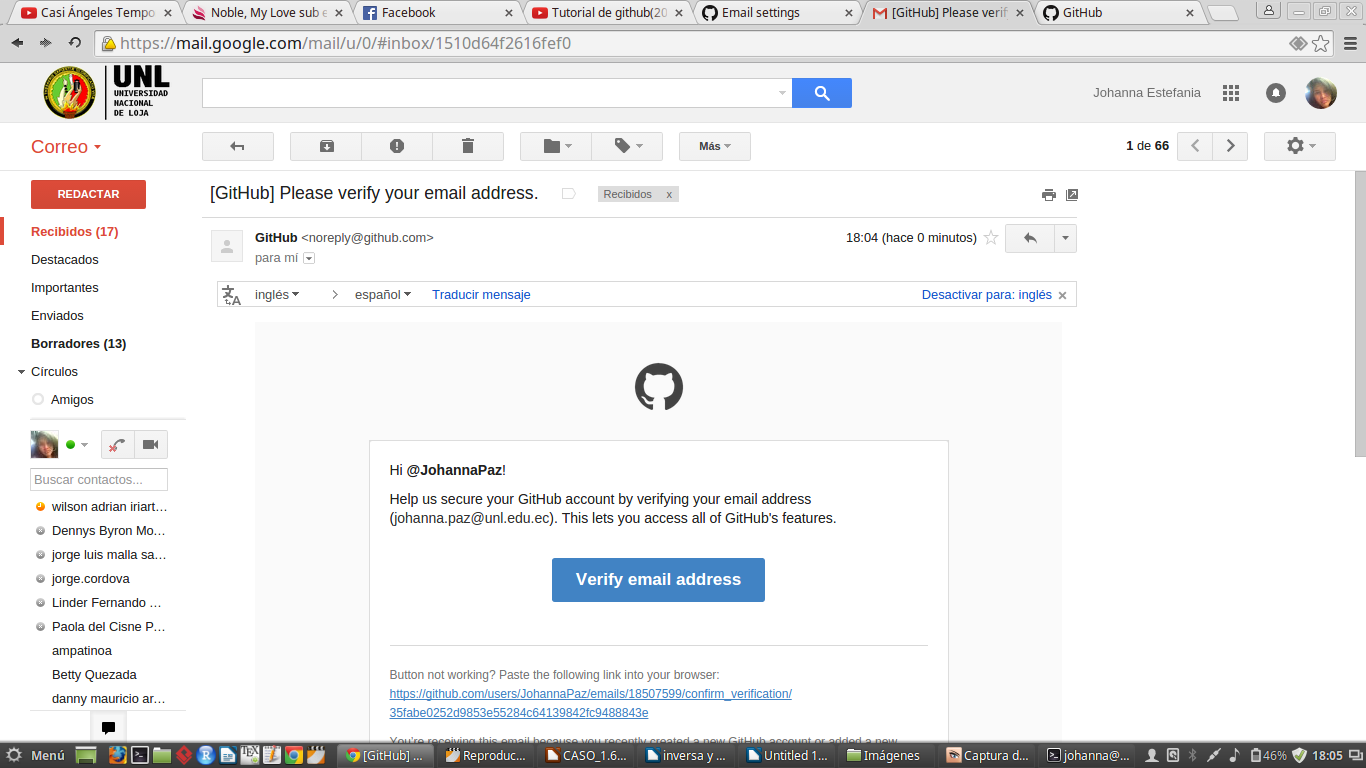
\includegraphics[width=8cm,height=5cm]{manual-img2.png}
		\end{center}
	\end{frame}

	\begin{frame}
		\frametitle{Instalación}
	\frametitle{Instalación}
		\begin{itemize}
			\item Ahora vamos a instalar Gihtub
			\item Abrimos una terminal para ejecutar el siguiente comando:
			\begin{center}
				 {\tt sudo apt-get install git-core}
			\end{center}	
		\end{itemize}
	\end{frame}	

	\begin{frame}
		\frametitle{Instalación}
		\begin{itemize}	
			\item Crear o ingresar en la carpeta que queremos clonar el repositorio
		\end{itemize}
		\begin{center}
			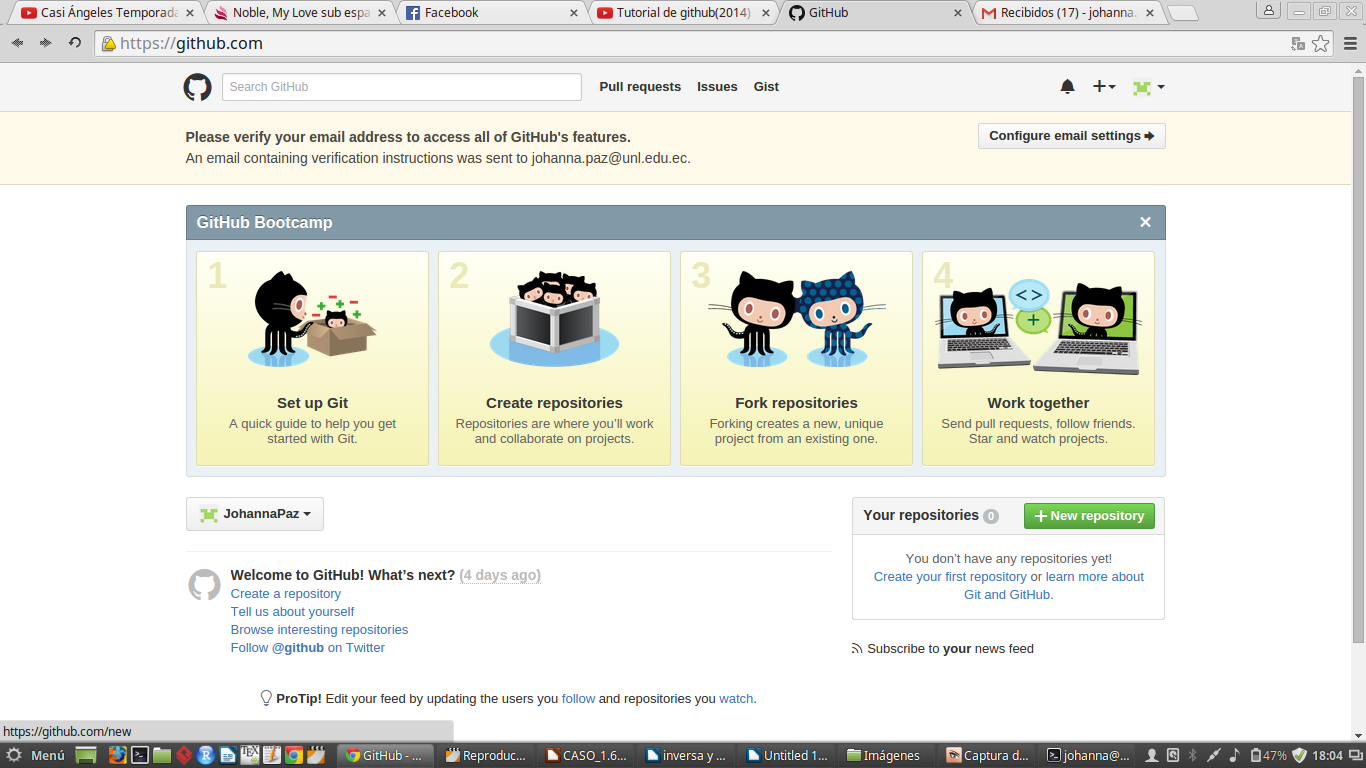
\includegraphics[width=8cm,height=5cm]{manual-img3.png}
		\end{center}
	\end{frame}
	
	\begin{frame}
		\frametitle{Instalación}
		Ahora vamos a crear el nuevo repositorio asi:
		\begin{center}
			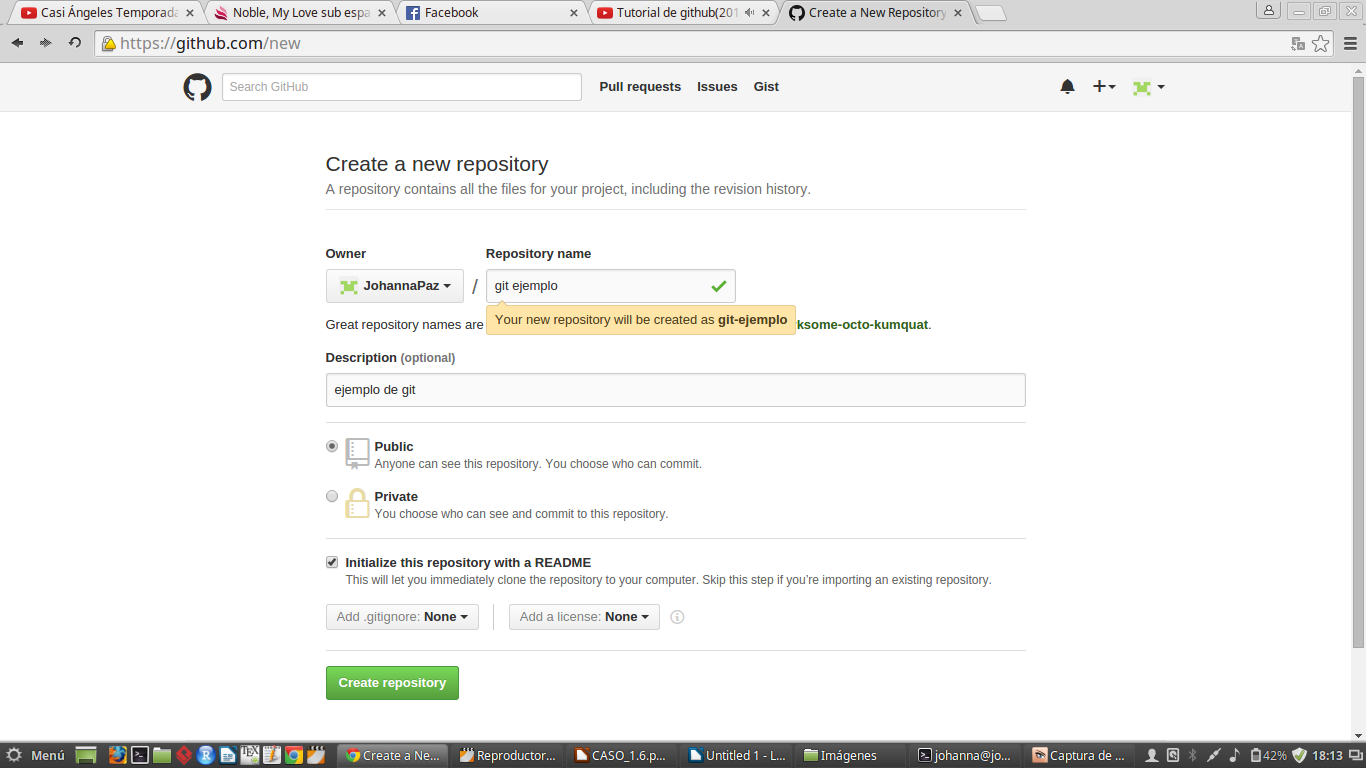
\includegraphics[width=8cm,height=5cm]{manual-img4.png}
		\end{center}
	\end{frame}

	\begin{frame}
		\frametitle{Instalación}
		\begin{itemize}
		\item Veamos como quedo creado el nuevo repositorio.\\
		git clone \url{https://github.com/JohannaPaz/git-ejemplo}
		\end{itemize}
		\begin{center}
			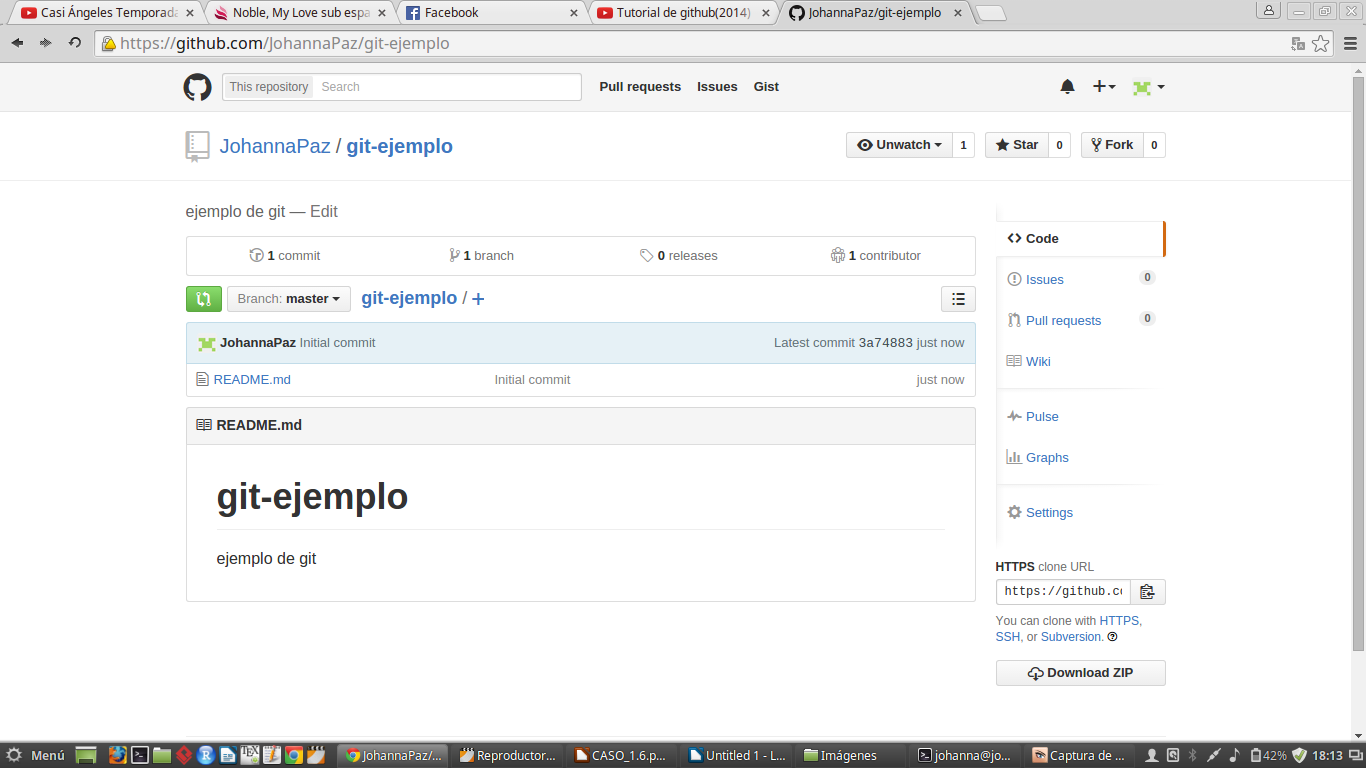
\includegraphics[width=8cm,height=5cm]{manual-img5.png}
		\end{center}
	\end{frame}

	\begin{frame}
		\frametitle{Instalación}
		{\small
		\begin{itemize}
			\item {\sffamily Una vez creado nuestro repositorio lo que tenemos que hacer es clonarlo.
			Para ello tenemos que crear una carpeta en cualquier lugar yo lo hecho así, la carpeta tiene el nombre de 				git proyecto}
		\end{itemize}}
		\begin{center}
			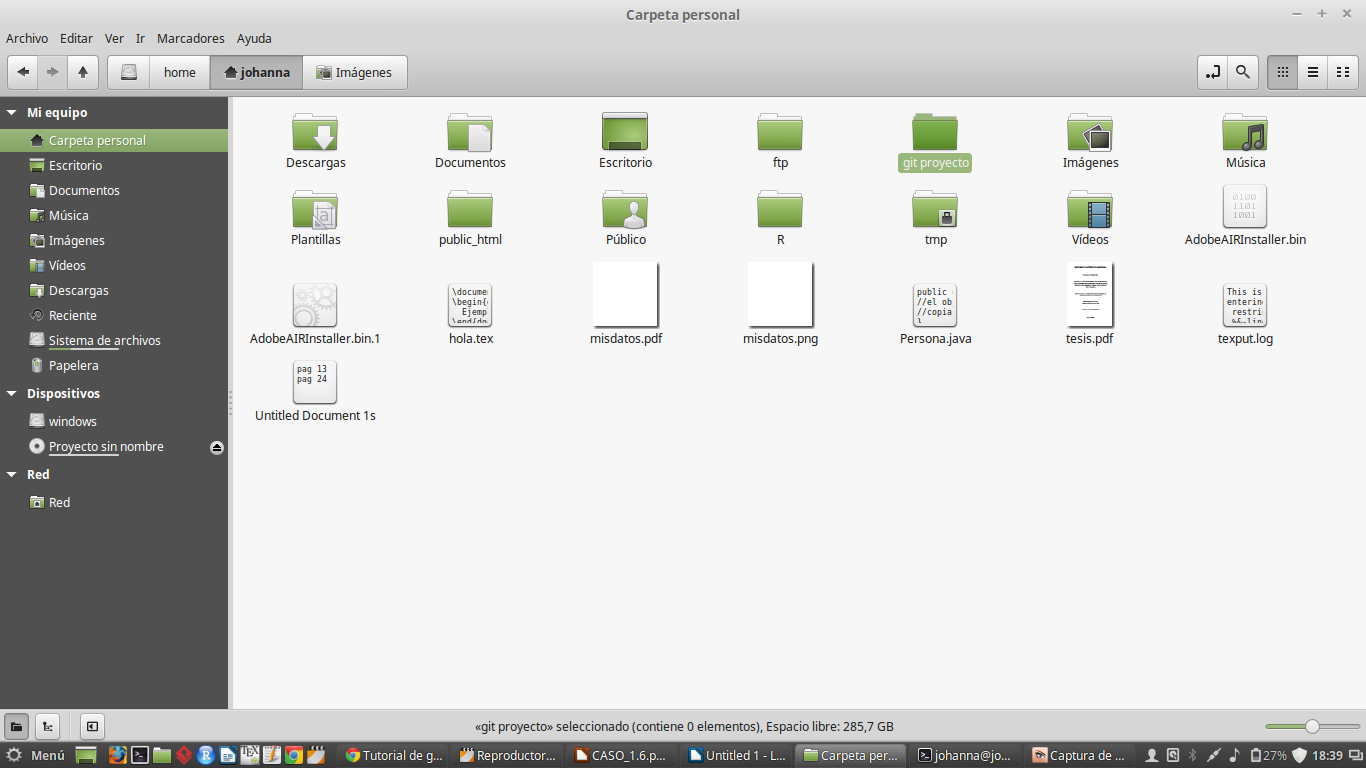
\includegraphics[width=8cm,height=5cm]{manual-img6.png}
		\end{center}
	\end{frame}
	\begin{frame}
		\frametitle{Instalación}
		\begin{itemize}
			\item Ahora accedemos a la consola y escribimos los siguientes comandos para
			poder clonar la carpeta:
			\begin{center}
				 {\tt \scriptsize cd git proyecto}\\
				 {\tt \scriptsize ls}\\
				 {\tt \scriptsize git clone https://github.com/JohannaPaz/git-ejemplo.git}\\
			\end{center}
		\end{itemize}
	\end{frame}

	\begin{frame}
		\frametitle{Instalación}
		\begin{itemize}
			\item Verificamos que se ha clonado la carpeta así:
		\end{itemize}
		\begin{center}
			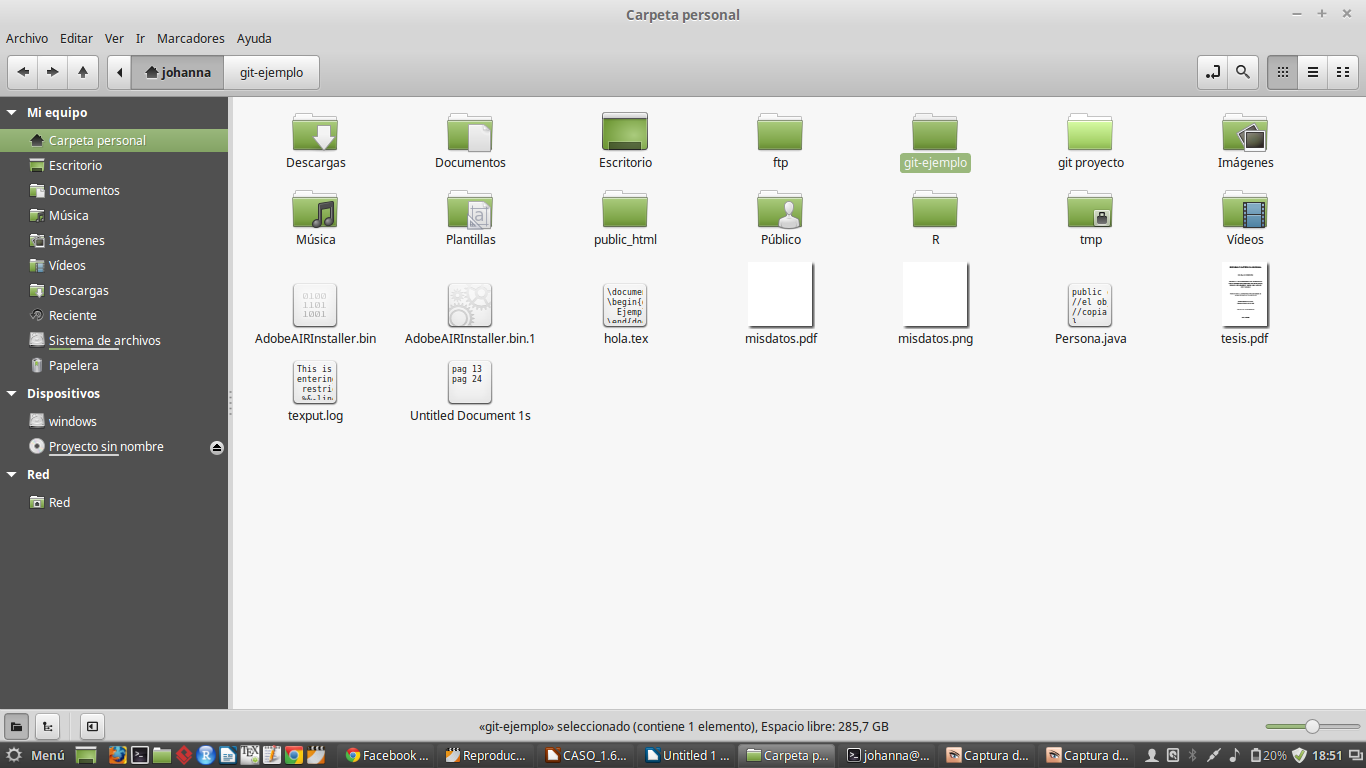
\includegraphics[width=8cm,height=5cm]{manual-img7.png}
		\end{center}
	\end{frame}
	
	\begin{frame}
		\frametitle{Instalación}
		\begin{itemize}
			\item Instalar git gui
			\begin{center}
				 {\tt \scriptsize sudo apt-get install gitk giggle git-cola git-gui gitg}\\
			\end{center}
			\item Abrir el gui de git mediante el comando, para eso tenemos q estar en
la carpeta donde clonamos el git. 
			\begin{center}
				 {\tt \scriptsize git gui}\\
			\end{center}
			\item Poner el nombre del usuario en git
			\begin{center}
				 {\tt \scriptsize git config -{}-global user.name nombre}\\	 
			\end{center}
			\item Colocar email del usuario
			\begin{center}
				 {\tt \scriptsize git config -{}-global user.email email}\\	 
			\end{center}
			\item Para asegurarnos de que no exista ning\'un cambio que nosotros notengamos.
			\begin{center}
				 {\tt \scriptsize git pull origin master}\\	 
			\end{center}
			\item Subimos los cambios.
			\begin{center}
				 {\tt \scriptsize git push origin master}\\	 
			\end{center}
		\end{itemize}
	\end{frame}

\subsection{Comandos}
	\begin{frame}
		\frametitle{Comandos Básicos}
		\begin{itemize}
			\item Inicializar repositorio git
			\begin{center}
				 {\tt \scriptsize git init}\\
			\end{center}
			\item Creación de un fichero README 
			\begin{center}
				 {\tt \scriptsize vi README.md}\\
			\end{center}
			\item Añadir a Git los ficheros modificados.
			\begin{center}
				 {\tt \scriptsize git add README.md}\\	 
			\end{center}
			\item Enviar los cambios hacia GitHub
			\begin{center}
				 {\tt \scriptsize git push origin master}\\	 
			\end{center}
		\end{itemize}
	\end{frame}
	\begin{frame}
		\frametitle{Ramas}
		Las ramas son utilizadas para desarrollar funcionalidades aisladas unas de otras.
		\begin{itemize}
			\item Crear una rama
			\begin{center}
				 {\tt \scriptsize git branch <nombre rama>}\\
			\end{center}
			\item Cambiar de rama
			\begin{center}
				 {\tt \scriptsize git checkout <nombre rama>}\\
			\end{center}
			\item Eliminar una rama
			\begin{center}
				 {\tt \scriptsize git branch -d <nombre rama>}\\	 
			\end{center}
			\item Renombrar una rama
			\begin{center}
				 {\tt \scriptsize git branch -m <vieja rama> <nueva rama>}\\	 
			\end{center}
		\end{itemize}
	\end{frame}
	\begin{frame}
		\frametitle{Acciones con Archivos}
		\begin{itemize}
			\item \textbf{Deshacer cambios locales (reset)}: Con este comando descartamos los cambios locales y volvemos al estado que teníamos guardado en el respositorio
			\begin{center}
				 {\tt \scriptsize git reset --hard}\\
			\end{center}
			\item Desahacer los cambios realizados en todos los archivos
			\begin{center}
				 {\tt \scriptsize git checkout -- .}\\
			\end{center}
			\item Actualizar repositorio local
			\begin{center}
				 {\tt \scriptsize git pull}\\	 
			\end{center}
			\item Fusionar ramas
			\begin{center}
				 {\tt \scriptsize git merge <branch>}\\	 
			\end{center}
			\item Crear una nueva etiqueta en este caso se llama 1.0.0
			\begin{center}
				 {\tt \scriptsize git tag 1.0.0 1b2e1d63ff}\\	 
			\end{center}
			\item Obtener el commit id
			\begin{center}
				 {\tt \scriptsize git log}\\	 
			\end{center}
		\end{itemize}
	\end{frame}

\subsection{Conclusiones}
\begin{frame}
\frametitle{Conclusiones}
	\begin{itemize}
			\item Es un excelente repositorio para el desrrollo en grupo.
			\item Podemos obtener conocimientos gracias a que es un repositorio donde se encuentra codigo profesional de manera gratuita.
			\item Podemos colaborar con el crecimeinto de sofware libre, subiendo nuestros codigos al repositorio.
		\end{itemize}
\end{frame}

\subsection{Bibliografía}
\begin{frame}
\frametitle{Bibliografia}
	\begin{enumerate}
		\item L. Castillo, Conociendo GitHub. \url{https://conociendogithub.readthedocs.org/en/latest/}.
		\item Y. Torregrosa, Álvaro.Luján Mora, Sergio,2013 \url{http://rua.ua.es/dspace/handle/10045/26796}.
		\item Ruiz, José Arístides Valencia.Revista San Gregorio,2015 \url{http://revista.sangregorio.edu.ec/index.php/RSANG/article/view/66}.
	\end{enumerate}
\end{frame}

\subsection{Licencia}
\begin{frame}
\frametitle{Licencia}
\begin{center}
\href{http://www.google.com}{
\includegraphics[scale=.8]{cc}}
\end{center}
\end{frame}

\MuchasGraciasFrame

\end{document}
